% 章节支持、单面打印:ctexbook
\documentclass[UTF8,AutoFakeBold,AutoFakeSlant,zihao=-4,oneside,openany]{ctexbook}
\usepackage[a4paper,left=3cm,right=2.6cm,top=3.5cm,bottom=2.9cm]{geometry}
% 目前 29mm 最接近 Word 排版


\usepackage{xeCJK}
\usepackage{titletoc}
\usepackage{fontspec}
\usepackage{setspace}
\usepackage{graphicx}
\usepackage{fancyhdr}
\usepackage{pdfpages}
\usepackage{booktabs}
\usepackage{multirow}
\usepackage{caption}
\usepackage{tikz}
\usepackage{etoolbox}
\usepackage{hyperref}
\usepackage{xcolor}
\usepackage{array}
\usepackage{amsmath}
\usepackage{amssymb}

% 设置超链接选项
\hypersetup{
  colorlinks=true,   % 启用链接的颜色
  linkcolor=blue,    % 目录跳转链接的颜色
  filecolor=magenta, % 本地文件链接颜色
  urlcolor=blue     % 网页链接颜色
}

% 让目录中的超链接没有框架和边框
\addtocontents{toc}{\protect\hypersetup{hidelinks}}


\usepackage[
  backend=biber,
  style=gb7714-2015,
  gbalign=gb7714-2015,
  gbnamefmt=lowercase,
  doi=false,
  url=false
]{biblatex}


\addbibresource{misc/ref.bib} % 参考文献引用文件位于 misc/ref.bib

% 字体设置
\setromanfont{Times New Roman}  % 西文字体默认为 Times New Roman
\newcommand{\xihei}{\heiti}

% 论文元数据
\newcommand{\thesisTitle}{论文(设计)题目:你的题目}
\newcommand{\thesisTitleEN}{题目英文名称:Your English Title}
\newcommand{\deptName}{计算机科学与技术学院}
\newcommand{\majorName}{人工智能}
\newcommand{\yourclass}{AI1111}
\newcommand{\yourName}{章三}
\newcommand{\yourStudentID}{24214234}
\newcommand{\mentorName}{李四}


% 主题页面格式:BIThesis
\fancypagestyle{BIThesis}{
  \setlength{\headheight}{20pt}   % 页眉高度
  \setlength{\footskip}{14pt}    % 页码高度

  \fancyhf{}    % 定义页眉、页码
  \fancyhead[L]{
\includegraphics[height=30pt]{images/logo.png}}
  \fancyhead[C]{\zihao{4}\ziju{0.08}\songti{贵州大学毕业论文(设计)}}
  \fancyhead[R]{\songti\zihao{5}第\thepage 页}
  \renewcommand{\headrulewidth}{0.6pt}    % 页眉分割线
}

% 设置章节格式
% 一级标题:黑体,三号,加粗;间距:段前 0.5 行,段后 1 行;
\ctexset{chapter={
    name = {第,章},
    number = {\arabic{chapter}},
    format = {\heiti \bfseries \centering \zihao{3}},
    aftername = \hspace{9bp},
    pagestyle = BIThesis,
    beforeskip = 8bp,
    afterskip = 32bp,
    fixskip = true,
  }
}

% 二级标题:黑体,四号,加粗;间距:段前 0.5 行,段后 0 行;
\ctexset{section={
    number = {\thechapter.\hspace{4bp}\arabic{section}},
    format = {\heiti \raggedright \bfseries \zihao{4}},
    aftername = \hspace{8bp},
    beforeskip = 20bp plus 1ex minus .2ex,
    afterskip = 18bp plus .2ex,
    fixskip = true,
  }
}

% 三级标题:黑体、小四、加粗;间距:段前 0.5 行,段后 0 行;
\ctexset{subsection={
    number = {\thechapter.\hspace{3bp}\arabic{section}.\hspace{3bp}\arabic{subsection}},
    format = {\heiti \bfseries \raggedright \zihao{-4}},
    aftername = \hspace{7bp},
    beforeskip = 17bp plus 1ex minus .2ex,
    afterskip = 14bp plus .2ex,
    fixskip = true,
  }
}

% 目录标题
\renewcommand{\contentsname}{
  \fontsize{16pt}{\baselineskip}
  \normalfont\heiti{目~~~~录}
  \vspace{-8pt}
}
% 定义目录样式
\titlecontents{chapter}[0pt]{\songti \zihao{-4}}
{\thecontentslabel\hspace{\ccwd}}{}
{\hspace{.5em}\titlerule*{.}\contentspage}
\titlecontents{section}[2\ccwd]{\songti \zihao{-4}}
{\thecontentslabel\hspace{\ccwd}}{}
{\hspace{.5em}\titlerule*{.}\contentspage}
\titlecontents{subsection}[4\ccwd]{\songti \zihao{-4}}
{\thecontentslabel\hspace{\ccwd}}{}
{\hspace{.5em}\titlerule*{.}\contentspage}

% 前置页面(原创性声明、中英文摘要、目录等)
\renewcommand{\frontmatter}{
  \pagenumbering{Roman}
  \setcounter{page}{0} 
  \pagestyle{BIThesis}
}

% 正文页面
\renewcommand{\mainmatter}{
  \pagenumbering{arabic}
  \pagestyle{BIThesis}
}

% 设置 caption 与 figure 之间的距离
\setlength{\abovecaptionskip}{11pt}
\setlength{\belowcaptionskip}{9pt}

% 设置图片的 caption 格式
\renewcommand{\thefigure}{\thechapter-\arabic{figure}}
\captionsetup[figure]{font=small,labelsep=space}

% 设置表格的 caption 与 table 之间的垂直距离
\captionsetup[table]{skip=2pt}

% 设置表格的 caption 格式
\renewcommand{\thetable}{\thechapter-\arabic{table}}
\captionsetup[table]{font=small,labelsep=space}

% 设置数学公式编号格式
\renewcommand{\theequation}{\arabic{chapter}-\arabic{equation}}

% 文档开始
\begin{document}
% 本页面为封面页,用于填写毕业论文的基本信息,一般不需要修改,可按需修改。

% Usage: \dunderline[<offset>]{<line_thickness>}
\newcommand\dunderline[3][-1pt]{{%
  \setbox0=\hbox{#3}
  \ooalign{\copy0\cr\rule[\dimexpr#1-#2\relax]{\wd0}{#2}}}}

% Cover Page
% Cover Page
\begin{titlepage}
  % 调整顶部间距
  \vspace*{0cm}  % 可根据需要减少初始间距

  \begin{tabular}{@{}c@{\hspace{0.5cm}}c@{}}
    
\includegraphics[width=0.23\textwidth]{images/logo.png} &
    
\includegraphics[width=0.47\textwidth]{images/header_gz.png} \\
  \end{tabular}

  \vspace*{1.2cm}  % 替代原来的-3mm
  % 标题部分保持不变
  \centering
  {\heiti\zihao{2}\ziju{0.12} 本科毕业论文(设计)}


  \vspace{2cm}

  \zihao{3}\textbf{\heiti\thesisTitle}

  \vspace{1.8cm}

  \flushleft
  \begin{spacing}{2}
    \hspace{27mm}\songti\zihao{3}\selectfont{学\hspace{11mm}院:
    \dunderline[-10pt]{1pt}{\makebox[78mm][c]{\deptName}}}

    \hspace{27mm}\songti\zihao{3}\selectfont{专\hspace{11mm}业:
    \dunderline[-10pt]{1pt}{\makebox[78mm][c]{\majorName}}}

    \hspace{27mm}\songti\zihao{3}\selectfont{班\hspace{11mm}级:
    \dunderline[-10pt]{1pt}{\makebox[78mm][c]{\yourclass}}}

    \hspace{27mm}\songti\zihao{3}\selectfont{学\hspace{11mm}号:
    \dunderline[-10pt]{1pt}{\makebox[78mm][c]{\yourStudentID}}}

    \hspace{27mm}\songti\zihao{3}\selectfont{学生姓名:
    \dunderline[-10pt]{1pt}{\makebox[78mm][c]{\yourName}}}

    \hspace{27mm}\songti\zihao{3}\selectfont{指导教师:
    \dunderline[-10pt]{1pt}{\makebox[78mm][c]{\mentorName}}}
  \end{spacing}

  \vspace{1.5cm}

  \centering
  \zihao{3}\ziju{0.5}\heiti\textbf{\today}
\end{titlepage}
 %封面页

% 前置页面定义
\frontmatter
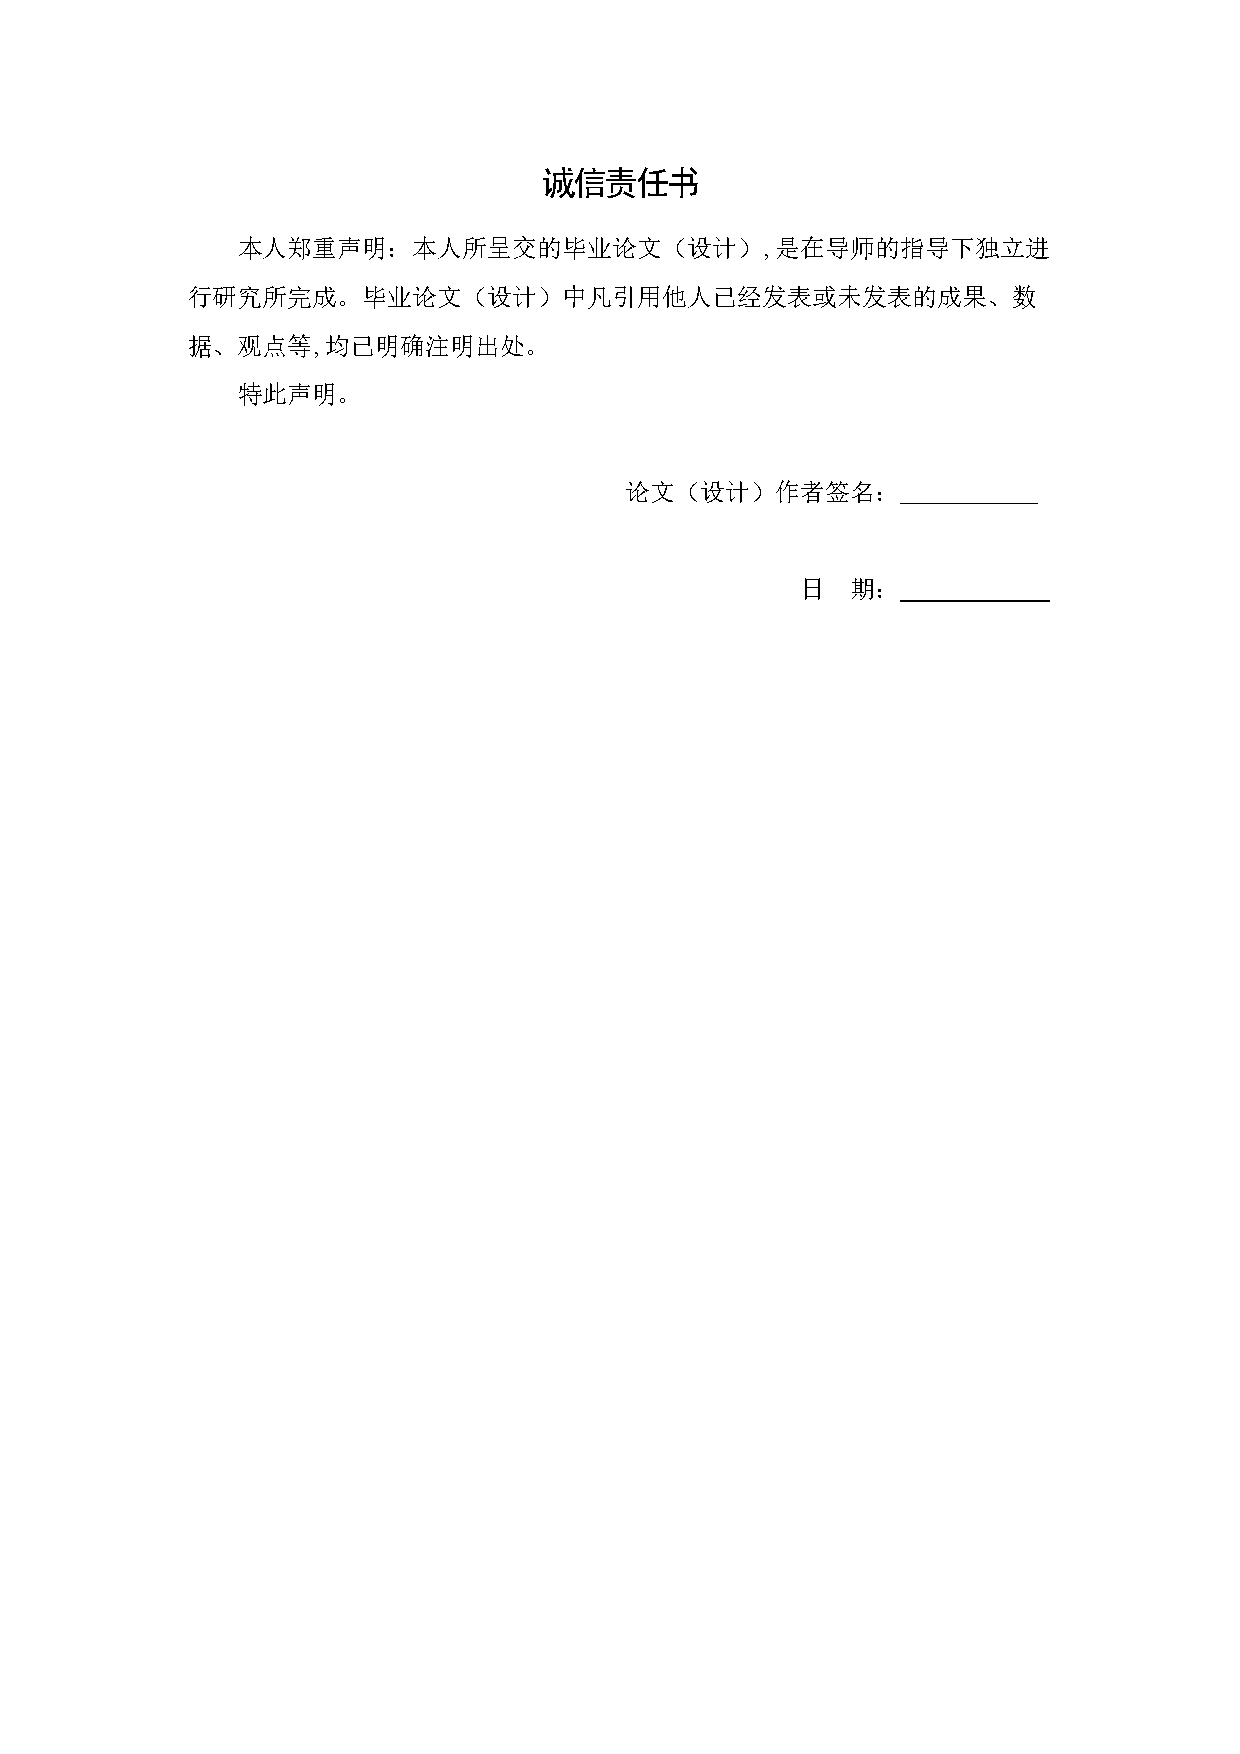
\includepdf{misc/1_commitment.pdf}  % 原创性声明:如无特殊需要,本部分无需改动
% 目录开始

% 调整目录行间距
\renewcommand{\baselinestretch}{1.35}
% 目录
\tableofcontents
\newpage
  % 目录页
% 中英文摘要章节
\topskip=0pt
\zihao{-4}

\vspace*{0mm}

\begin{center}
  \heiti\zihao{-2}\textbf{\thesisTitle}
\end{center}

\vspace*{2mm}


{\let\clearpage\relax 
\chapter*{摘~~~~要}
\addcontentsline{toc}{chapter}{摘~~~~要}}

\vspace*{2mm}

\setstretch{1.53}
\setlength{\parskip}{0em}

% 中文摘要正文从这里开始

中文摘要正文从这里开始\par
\vspace{4ex}\noindent\textbf{\heiti 关键词:大模型、RAG、VOSK、ROS机器人、SLAM、融合建图}
\newpage

% 英文摘要章节
\topskip=0pt

\vspace*{2mm}

\begin{spacing}{0.95}
  \centering
  \heiti\zihao{3}\textbf{\thesisTitleEN}
\end{spacing}

\vspace*{17mm}

{\let\clearpage\relax 
\chapter*{Abstract}
\addcontentsline{toc}{chapter}{Abstract}
}

\setstretch{1.53}
\setlength{\parskip}{0em}

% 英文摘要正文从这里开始

英文摘要正文从这里开始\par
\vspace{3ex}\noindent\textbf{Key Words: Large language models (LLMs), RAG, VOSK, ROS-based robotics, SLAM, integrated mapping}
\newpage


 % 中英文摘要页



% 正文开始
\mainmatter
\setlength{\parskip}{0em} % 正文 22 磅的行距
\renewcommand{\baselinestretch}{1.53}

% 第一章
% 第一章
\chapter{绪论}
\section{研究背景及意义}
**************************************************
\section{国内外研究现状}
\subsection{国外研究现状}
************引用文献\cite{quigley2009ros},
***********\cite{piastou2025efficiency}。****
\subsection{国内研究现状}
*****************
\section{本文主要内容}
*******************

% 第二章

\chapter{技术概述}

\section{大模型}
*********
\subsection{asdasd}
*********引用图片\ref{fig:transformer}\parencite[postnote]{bibid}
\begin{figure}[htbp]
	\vspace{13pt} % 调整图片与上文的垂直距离
	\centering
	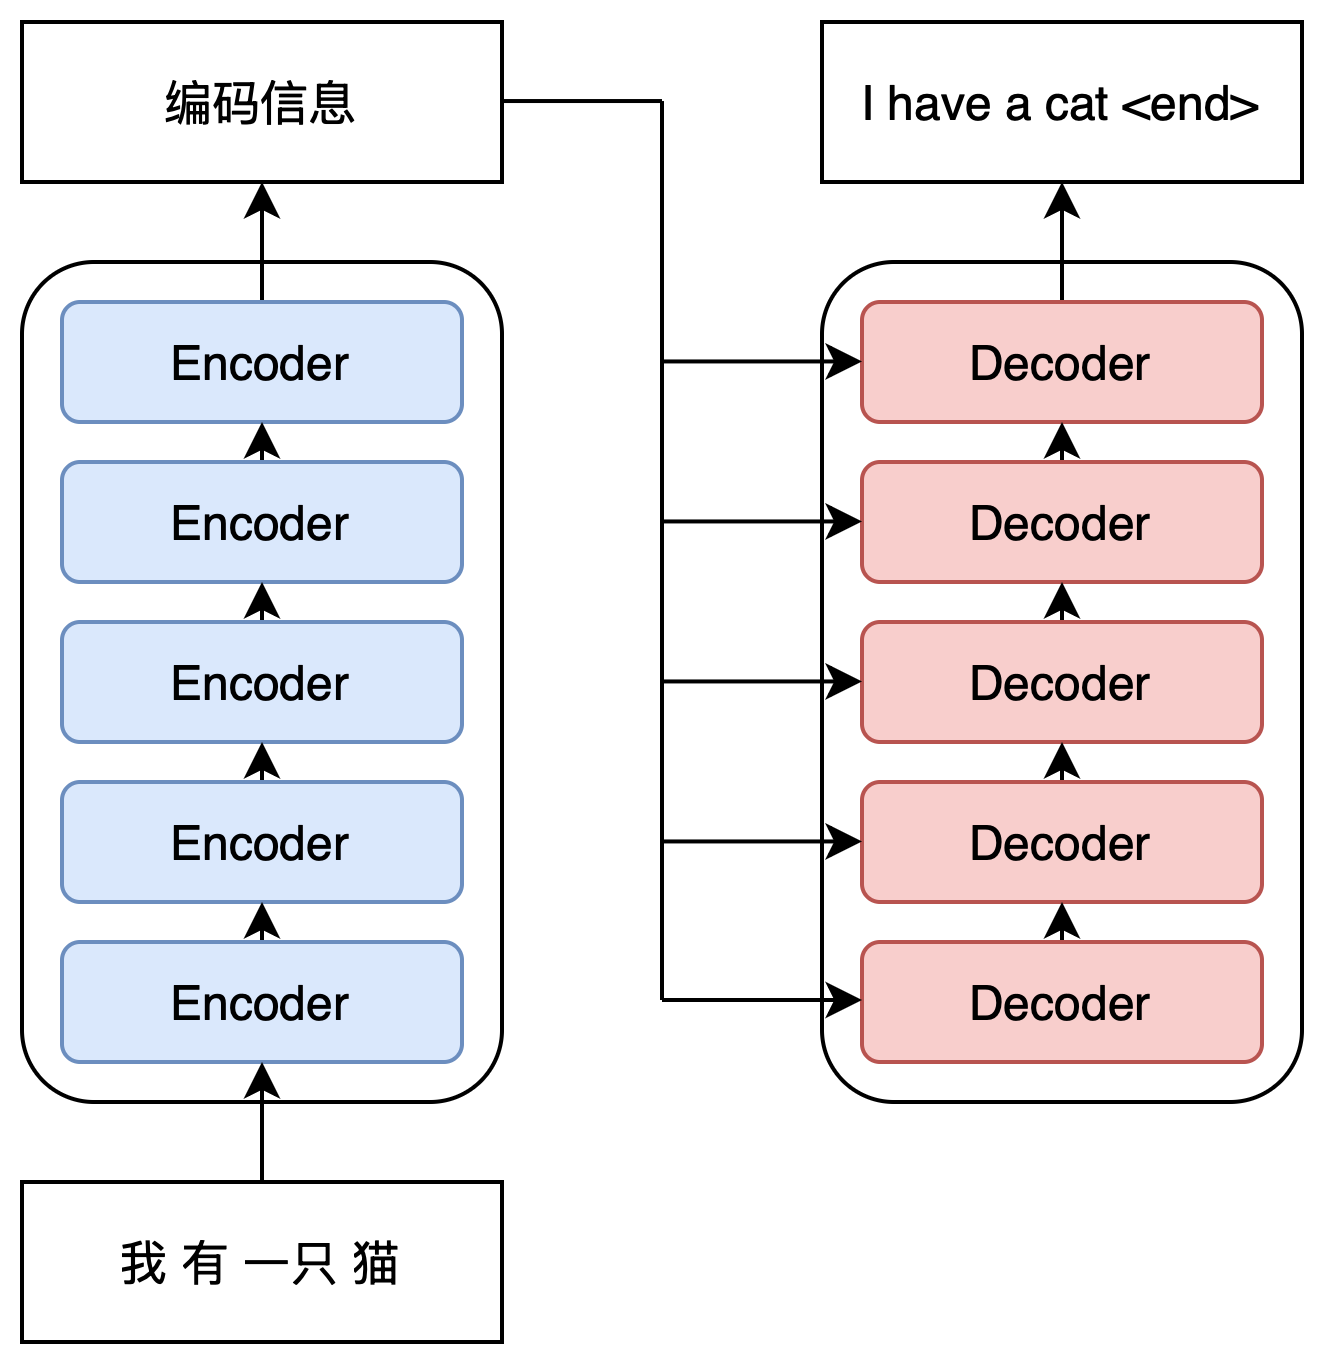
\includegraphics[]{images/Transformer.png}
	\caption{Transformer架构图}\label{fig:transformer} % label 用来在文中索引
\end{figure}

****************




% 结尾
\addcontentsline{toc}{chapter}{结束语}
\chapter*{\vskip 10bp\textmd{结束语} \vskip -6bp}

% 在结论部分的子标题不需要序号,加上 * 即可(一个例子如下)
% \section*{结论段落标题}

% 这里插入一个参考文献,仅作参考


\textcolor{blue}{结论作为毕业设计(论文)正文的最后部分单独排写,但不加章号。结论是对整个论文主要结果的总结。在结论中应明确指出本研究的创新点,对其应用前景和社会、经济价值等加以预测和评价,并指出今后进一步在本研究方向进行研究工作的展望与设想。结论部分的撰写应简明扼要,突出创新性。阅后删除此段。}

\textcolor{blue}{结论正文样式与文章正文相同:宋体、小四;行距:22 磅;间距段前段后均为 0 行。阅后删除此段。}
 % 结束页
% 参考文献开始
% \addcontentsline{toc}{chapter}{参考文献}
% \chapter*{\vskip 10bp \textmd{参考文献} \vskip -6bp}

% 设置参考文献字号为 5 号
\renewcommand*{\bibfont}{\zihao{5}}
% 设置参考文献各个项目之间的垂直距离为 0
\setlength{\bibitemsep}{0ex}
\setlength{\bibnamesep}{0ex}
\setlength{\bibinitsep}{0ex}
% 设置单倍行距
\renewcommand{\baselinestretch}{1.2}
% 设置参考文献顺序标签 `[1]` 与文献内容 `作者. 文献标题...` 的间距
\setlength{\biblabelsep}{-2mm}
\settowidth{\labelwidth}{\mkbibbrackets{999}\hspace{\biblabelsep}}
% 设置整体缩进 = 标签宽度 + 标签后间距
\setlength{\bibhang}{\labelwidth}
% 设置参考文献后文缩进为 0(与 Word 模板保持一致)
\DeclareFieldFormat{labelnumberwidth}{\mkbibbrackets{#1}}
\DeclareFieldFormat{bibentrysetflag}{\mbox{}}


\renewcommand{\itemcmd}{%
  \makebox[\labelwidth][l]{\mkbibbrackets{\printfield{labelnumber}}}%
  \hspace{\biblabelsep}%
}


% 删除默认的「参考文献 / Reference」标题,使用上面定义的 section 标题

\printbibliography


 % 参考文献页
% 附录
\addcontentsline{toc}{chapter}{附~~~~录}
\chapter*{\vskip 10bp \textmd{附~~~~录} \vskip -6bp}

附录相关内容…

\textcolor{blue}{附录是毕业设计(论文)主体的补充项目,为了体现整篇文章的完整性,写入正文又可能有损于论文的条理性、逻辑性和精炼性,这些材料可以写入附录段,但对于每一篇文章并不是必须的。附录依次用大写正体英文字母 A、B、C……编序号,如附录 A、附录 B。阅后删除此段。}

\textcolor{blue}{附录正文样式与文章正文相同:宋体、小四;行距:22 磅;间距段前段后均为 0 行。阅后删除此段。}
 % 附录页
% 请在此处添加致谢内容

\addcontentsline{toc}{chapter}{致~~~~谢}
\chapter*{\vskip 10bp \textmd{致~~~~谢} \vskip -6bp}

值此论文完成之际,首先向我的导师……

\textcolor{blue}{致谢正文样式与文章正文相同:宋体、小四;行距:22 磅;间距段前段后均为 0 行。阅后删除此段。}
 % 致谢页
\end{document}
